\chapter{Исследовательская часть}

В данном разделе будет приведен пример работы программы, а также проведен сравнительный анализ алгоритмов при различных ситуациях на основе полученных данных.

\section{Технические характеристики}

Технические характеристики устройства, на котором выполнялись замеры по времени представлены далее.

\begin{itemize}
	\item Процессор: Intel(R) Core(TM) i7-1165G7 CPU 2.80 ГГц.
	\item Количество ядер: 4 физических и 8 логических.
	\item Оперативная память: 15 ГБайт.
	\item Операционная система: Ubuntu 64-разрядная система версии 22.04.3.
\end{itemize}

При замерах времени ноутбук был включен в сеть электропитания и был нагружен только системными приложениями.

\section{Демонстрация работы программы}

На рисунке~\ref{img:example}  представлен пример работы программы для обоих алгоритмов --- полного перебора и муравьиного.
Осуществляется выбор файла с данными, ввод коэффициентов для муравьиного алгоритма, а также выполнение алгоритма решения задачи коммивояжера методом полного перебора и методом на основе муравьиного алгоритма.

\clearpage

\begin{figure}[h]
	\centering
	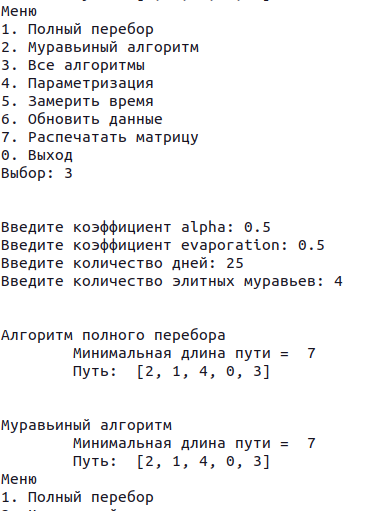
\includegraphics[width=0.5\textwidth]{img/example.png}
	\caption{Пример работы программы}
	\label{img:example}
\end{figure}

\section{Временные характеристики}

Для замеров времени используется функция \textit{process\_time(...)} из библиотеки \textit{time} для \textit{Python}.
Функция возвращает процессорное время в секундах.

Замеры проводились для разного размера матриц, чтобы определить, когда наиболее эффективно использовать муравьиный алгоритм.

Результаты замеров приведены в таблице \ref{tbl:time} (время в секундах).

\clearpage

\begin{table}[ht]
	\small
	\begin{center}
		\begin{threeparttable}
		\caption{Результаты замеров времени (в с.)}
		\label{tbl:time}
		\begin{tabular}{|c|c|c|}
			\hline
			\multirow{2}{*}{\bfseries Размер матрицы} & \multicolumn{2}{c|}{\bfseries Время, мкс} \\ \cline{2-3}
			 & \bfseries Полный перебор & \bfseries Полный перебор
			\csvreader{csv/times.csv}{}
			{\\\hline \csvcoli & \csvcolii & \csvcoliii } \\
			\hline
		\end{tabular}
		\end{threeparttable}
	\end{center}
\end{table}

На рисунке~\ref{img:g1} приведен график результатов замеров времени работы реализаций алгоритмов для различных линейных размеров
матриц.

\begin{figure}[h!]
	\centering
	\begin{tikzpicture}
		\begin{axis}[
			height = 0.4\paperheight,
			width = 0.7\paperwidth,
			legend pos = north west,
			table/col sep=comma,
			xlabel={размер матрицы},
			ylabel={время, мкс},
			xmin=1.9,
			xmax=9,
			]
			\legend{
				Полный перебор,
				Муравьиный,
			};
			\addplot [
			solid,
			thick,
			draw = blue,
			mark = --,
			mark options = {
				scale = 2,
				fill = blue,
				draw = black
			}
			] table [x=size, y=full] {csv/times.csv};
			\addplot [
			dashed,
			thick,
			draw = red,
			mark = --,
			mark options = {
				scale = 2,
				fill = blue,
				draw = black
			}
			] table [x=size, y=ants] {csv/times.csv};
			{csv/times.csv};
		\end{axis}
	\end{tikzpicture}
	\caption{Результаты замеров времени работы реализации для различных размеров матриц}
	\label{img:g1}
\end{figure}

\clearpage

\section{Постановка эксперимента}

Автоматическая параметризация была проведена на трех классах данных.
Алгоритм будет запущен для набора значений $\alpha, \rho \in (0, 1)$, $\text{Elites} \in (0, 1, 3, 6), t_{max1} = 500, t_{max2} = 5000$, где $t_{max1}$ использовался для первого класса данных, $t_{max2}$ использовался для второго.
Количество дней всегда равно 100.

Итоговая таблица значений параметризации будет состоять из следующих колонок:
\begin{itemize}[label=---]
	\item $\alpha$ --- коэффициент жадности;
	\item $\rho$ --- коэффициент испарения;
	\item \textit{Elites} --- количество элитных муравьев;
	\item \textit{Mistake} --- разность полученного основанным на муравьином алгоритме методом значения и эталонного значения на данных значениях параметров, показатель качества решения.
\end{itemize}

Цель эксперимента --- определить комбинацию параметров, которые позволяют решить задачу с наименьшим значением ошибки для выбранного класса данных.
Качество решения зависит от погрешности измерений.

\subsection{Класс данных 1}\label{par:class1}

Класс данных 1 представляет собой 3 матрицы смежности для 10 вершин (небольшой разброс длины пути --- от 10 до 50), каждая из которых представлена далее.

\begin{equation}
	\label{eq:kd1.1}
	K_{1.1} = \begin{pmatrix}
		0 & 22 & 11 & 30 & 25 & 16 & 41 & 28 & 26 & 35 \\
		40 & 0 & 16 & 15 & 26 & 30 & 13 & 11 & 33 & 17 \\
		24 & 23 & 0 & 29 & 25 & 18 & 12 & 42 & 31 & 35 \\
		10 & 50 & 27 & 0 & 45 & 29 & 41 & 40 & 30 & 20 \\
		31 & 29 & 14 & 14 & 0 & 29 & 26 & 21 & 37 & 21 \\
		25 & 11 & 13 & 23 & 42 & 0 & 14 & 22 & 34 & 23 \\
		12 & 28 & 39 & 37 & 45 & 41 & 0 & 23 & 32 & 20 \\
		17 & 35 & 42 & 19 & 25 & 32 & 44 & 0 & 28 & 16 \\
		38 & 47 & 18 & 30 & 24 & 16 & 32 & 33 & 0 & 22 \\
		33 & 48 & 42 & 23 & 41 & 35 & 43 & 24 & 31 & 0 \\
	\end{pmatrix}
\end{equation}

\begin{equation}
	\label{eq:kd1.2}
	K_{1.2} = \begin{pmatrix}
		0 & 10 & 31 & 13 & 36 & 26 & 40 & 25 & 48 & 24 \\
		42 & 0 & 50 & 46 & 32 & 48 & 49 & 15 & 19 & 18 \\
		37 & 48 & 0 & 47 & 41 & 22 & 22 & 50 & 32 & 11 \\
		22 & 23 & 35 & 0 & 17 & 48 & 37 & 34 & 50 & 25 \\
		14 & 15 & 45 & 43 & 0 & 19 & 13 & 16 & 25 & 39 \\
		25 & 36 & 16 & 25 & 38 & 0 & 46 & 45 & 32 & 37 \\
		20 & 22 & 17 & 33 & 50 & 49 & 0 & 49 & 28 & 39 \\
		27 & 34 & 12 & 14 & 37 & 32 & 35 & 0 & 34 & 13 \\
		50 & 35 & 33 & 46 & 34 & 24 & 41 & 13 & 0 & 35 \\
		18 & 47 & 39 & 43 & 36 & 38 & 23 & 50 & 44 & 0 \\
	\end{pmatrix}
\end{equation}

\begin{equation}
	\label{eq:kd1.3}
	K_{1.3} = \begin{pmatrix}
		0 & 42 & 36 & 15 & 22 & 19 & 38 & 32 & 19 & 23 \\
		38 & 0 & 26 & 27 & 36 & 19 & 36 & 16 & 26 & 18 \\
		25 & 29 & 0 & 45 & 22 & 18 & 12 & 40 & 43 & 20 \\
		11 & 22 & 21 & 0 & 35 & 49 & 16 & 34 & 24 & 19 \\
		26 & 45 & 28 & 30 & 0 & 47 & 29 & 33 & 36 & 31 \\
		37 & 50 & 17 & 18 & 43 & 0 & 39 & 45 & 34 & 18 \\
		17 & 39 & 39 & 39 & 38 & 43 & 0 & 30 & 19 & 40 \\
		48 & 35 & 29 & 24 & 39 & 31 & 42 & 0 & 40 & 27 \\
		44 & 40 & 48 & 35 & 23 & 25 & 44 & 49 & 0 & 18 \\
		25 & 40 & 11 & 41 & 16 & 28 & 20 & 46 & 17 & 0 \\
	\end{pmatrix}
\end{equation}

Для данного класса данных параметризация приведена в приложении А.
Для каждого набора параметров в качестве разности указано максимальное полученное значение отклонения для всех матриц данного класса при указанных параметрах.

Лучшими наборами этого класса являются $(\alpha = 0.5, \rho = 0.3, \text{Elites} = \text{любое})$, $(\alpha = 0.4, \rho = 0.7, \text{Elites} = \text{любое})$, $(\alpha = 0.7, \rho = 0.7, \text{Elites} = \text{любое})$, $(\alpha = 0.8, \rho = 0.2, \text{Elites} = \text{любое})$.
При этих значениях $\alpha$ и $\rho$ ошибка принимает значения 0 или 1 при любом количестве элитных муравьев, из-за чего рекомендуется использовать именно эти значения.

Корреляцию между количеством элитных муравьев и погрешностью найти не удалось.

\subsection{Класс данных 2}\label{par:class2}

Класс данных 2 представляет собой 3 матрицы смежности для 10 вершин (большой разброс значений длины пути - от 100 до 999), каждая из которых представлена далее.

\begin{equation}
	\label{eq:kd2.1}
	K_{2.1} = \begin{pmatrix}
        0 & 551 & 637 & 618 & 475 & 983 & 397 & 818 & 507 & 173 \\
        747 & 0 & 340 & 686 & 173 & 433 & 871 & 636 & 194 & 357 \\
        599 & 405 & 0 & 108 & 737 & 555 & 145 & 527 & 428 & 329 \\
        470 & 344 & 193 & 0 & 192 & 403 & 223 & 900 & 285 & 974 \\
        632 & 613 & 841 & 994 & 0 & 547 & 644 & 375 & 590 & 437 \\
        596 & 358 & 636 & 467 & 848 & 0 & 922 & 998 & 218 & 875 \\
        742 & 962 & 424 & 858 & 219 & 481 & 0 & 596 & 320 & 117 \\
        685 & 712 & 897 & 535 & 868 & 547 & 953 & 0 & 271 & 935 \\
        388 & 110 & 571 & 563 & 454 & 537 & 258 & 406 & 0 & 399 \\
        964 & 484 & 426 & 817 & 216 & 752 & 304 & 730 & 693 & 0 \\
	\end{pmatrix}
\end{equation}

\begin{equation}
	\label{eq:kd2.2}
	K_{2.2} = \begin{pmatrix}
		0 & 854 & 112 & 569 & 144 & 102 & 788 & 751 & 295 & 138 \\
		819 & 0 & 741 & 419 & 346 & 945 & 285 & 791 & 185 & 934 \\
		299 & 150 & 0 & 542 & 631 & 650 & 325 & 406 & 801 & 838 \\
		817 & 505 & 575 & 0 & 123 & 582 & 290 & 518 & 627 & 755 \\
		886 & 151 & 497 & 271 & 0 & 409 & 799 & 180 & 891 & 468 \\
		838 & 503 & 954 & 322 & 311 & 0 & 878 & 158 & 832 & 995 \\
		141 & 972 & 339 & 882 & 305 & 100 & 0 & 157 & 781 & 153 \\
		756 & 188 & 442 & 902 & 393 & 242 & 974 & 0 & 859 & 196 \\
		552 & 168 & 668 & 298 & 322 & 663 & 405 & 186 & 0 & 658 \\
		396 & 847 & 630 & 895 & 742 & 560 & 713 & 894 & 180 & 0 \\
	\end{pmatrix}
\end{equation}

\begin{equation}
	\label{eq:kd2.3}
	K_{2.3} = \begin{pmatrix}
		0 & 814 & 726 & 929 & 155 & 509 & 211 & 790 & 808 & 917 \\
		317 & 0 & 739 & 648 & 955 & 766 & 390 & 560 & 900 & 734 \\
		435 & 467 & 0 & 557 & 406 & 424 & 994 & 803 & 424 & 268 \\
		324 & 896 & 988 & 0 & 712 & 877 & 455 & 435 & 866 & 478 \\
		481 & 572 & 388 & 956 & 0 & 393 & 766 & 566 & 128 & 961 \\
		690 & 710 & 278 & 591 & 587 & 0 & 293 & 461 & 124 & 280 \\
		778 & 637 & 384 & 567 & 332 & 241 & 0 & 594 & 755 & 209 \\
		988 & 611 & 661 & 598 & 400 & 409 & 956 & 0 & 517 & 229 \\
		610 & 375 & 922 & 256 & 169 & 448 & 477 & 834 & 0 & 665 \\
		235 & 829 & 888 & 327 & 888 & 965 & 566 & 722 & 599 & 0 \\
	\end{pmatrix}
\end{equation}


Для данного класса данных параметризация приведена в приложении Б.
Для каждого набора параметров в качестве разности указано максимальное полученное значение отклонения для всех матриц данного класса при указанных параметрах.

Лучшими наборами этого класса являются $(\alpha = 0.6, \rho = 0.2, \text{Elites} = \text{любое})$
При этих значениях $\alpha$ и $\rho$ ошибка принимает значение 0 при любом количестве элитных муравьев, из-за чего рекомендуется использовать именно эти значения.

Корреляцию между количеством элитных муравьев и погрешностью найти не удалось.

\section*{Вывод}

В результате эксперимента было получено, что использование муравьиного алгоритма наиболее эффективно для матриц, размер которых превышает 8.
Так, при размере матрицы равном 2, муравьиный алгоритм медленее алгоритма полного перебора в 143 раза, а при размере матрицы, равном 8, муравьиный алгоритм быстрее алгоритма полного перебора в 11 раз, а при размере в 10 -- уже в 15 раз.
Следовательно, при размерах матриц больше 8 следует использовать муравьиный алгоритм, но стоит учитывать, что он не гарантирует получение минимального результата при решении задачи.

Также при проведении эксперимента с классами данных было получено, что на первом классе данных муравьиный алгоритм лучше всего показывает себя при параметрах:
\begin{itemize}[label=---]
	\item $\alpha = 0.5, \rho = 0.3, \text{Elites} = \text{любое}$;
	\item $\alpha = 0.4, \rho = 0.7, \text{Elites} = \text{любое}$;
	\item $\alpha = 0.7, \rho = 0.7, \text{Elites} = \text{любое}$;
	\item $\alpha = 0.8, \rho = 0.2, \text{Elites} = \text{любое}$;
\end{itemize}

Для класса данных 1 рекомендуется использовать данные параметры.

Для класса данных 2 было получено, что с наименьшим значением ошибки алгоритм работает при значениии параметров $\alpha = 0.6, \rho = 0.2, \text{Elites} = \text{любое}$.
Для класса данных 2 рекомендуется использовать данные параметры.

Корреляцию между количеством элитных муравьев и погрешностью найти не удалось ни для одного из классов данных.
